% Supplementary material for the JBHI manuscript (jbhi_compact.tex). Every number is checked against results/ by
% paper/audit_jbhi_numbers.py, which reads this file together with the manuscript.
\documentclass[journal]{IEEEtran}
\usepackage{amsmath,amssymb,amsthm}
\usepackage{graphicx}
\usepackage{booktabs}
\usepackage{array}
\newcolumntype{L}[1]{>{\raggedright\arraybackslash}p{#1}}
\usepackage{cite}
\usepackage{url}
\usepackage[hidelinks]{hyperref}
\renewcommand{\thesection}{S\arabic{section}}
\renewcommand{\thetable}{S\arabic{table}}
\renewcommand{\thefigure}{S\arabic{figure}}
\renewcommand{\theequation}{S\arabic{equation}}
\newtheorem{assumption}{Assumption}
\setcounter{assumption}{1}
\newtheorem*{prop4}{Proposition 4 (restated)}
\newcommand{\Prb}{\mathbb{P}}

\begin{document}
\title{Supplementary Material for ``Certified Adaptive Examination of Blood Smears: Why Information-Gain Stopping Cannot Certify Rare Evidence, and What Can Be Guaranteed Instead''}
\author{Qudrat~Ullah and Bal\'azs~Harangi}
\markboth{IEEE Journal of Biomedical and Health Informatics}{Ullah and Harangi: Supplementary Material}
\maketitle

\noindent Sections, figures and tables of the manuscript are cited by their numbers there. Analyses marked exploratory were not pre-registered; scripts, seeds and results are in the repository named in the manuscript.

\section{Certifying absence (RQ2)}
Fig.~\ref{fig:partII} shows the fraction of fields that any strategy without location information must examine to certify the absence of $k$ critical fields (Theorem~1 and Proposition~1). For $N=1{,}000$ and $\alpha=0.05$ this is 950 fields for $k=1$, 450 for $k=5$ and 258 for $k=10$; the sufficient closed form $N(1-\alpha^{1/k})$ gives 950, 451 and 259.

\begin{figure}[t]
\centering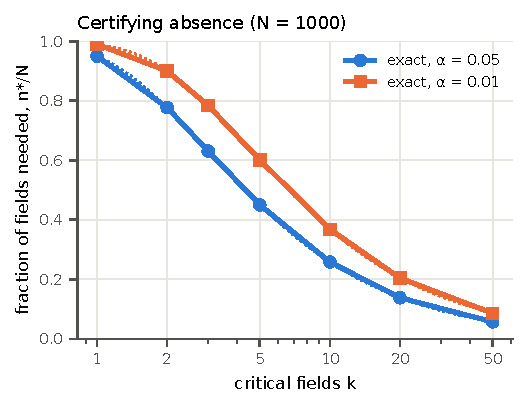
\includegraphics[width=0.72\columnwidth]{figures/fig2_partII.pdf}
\caption{Fraction of fields that any strategy without location information must examine to certify the absence of $k$ critical fields ($N=1000$; exact values solid, sufficient closed form $1-\alpha^{1/k}$ dotted).}\label{fig:partII}
\end{figure}

\section{Proposition 4: proof and numbers (RQ3)}
\subsection{Setting}
A specimen has $M$ cells with labels $L\in\{0,1\}^M$ (1: blast), $B=\sum_iL_i$ blasts and $p=B/M$. The examiner sees side information $S$ (positions, images, classifier scores, anything) and has independent randomization $U$. A procedure verifies distinct cells $I_1,I_2,\dots$, where $I_t$ is a function of $(S,U,I_1,L_{I_1},\dots,I_{t-1},L_{I_{t-1}})$; it stops at a stopping time $\tau$ of the filtration $\mathcal F_t=\sigma(S,U,(I_s,L_{I_s})_{s\le t})$ and outputs an $\mathcal F_\tau$-measurable decision $D\in\{\text{certify},\text{not}\}$. It is \emph{valid at level $\alpha$} for $H_0:p\le\theta$ if $\Prb_U(D=\text{certify})\le\alpha$ for every fixed population $(S,L)$ with $B\le\theta M$.

\begin{assumption}[No information about labels]\label{as:noinfo}
Under the model $\Prb_B$, $L$ is uniformly distributed over the $\binom MB$ arrangements with $B$ blasts and independent of $(S,U)$.
\end{assumption}
Assumption~1 of Theorem~1 is the analogue for the absence problem. Let $B_0=\lfloor\theta M\rfloor$, $X_n\sim\mathrm{Hyp}(M,B,n)$ the number of blasts in $n$ uniform draws without replacement, and $\beta^*_n(B)$ the power at $B$ of the randomized test of $B_0$ that rejects when $X_n>c$, and with probability $\gamma$ when $X_n=c$, where $\Prb_{B_0}(X_n>c)+\gamma\Prb_{B_0}(X_n=c)=\alpha$.

\begin{prop4}
Under Assumption~\ref{as:noinfo}, for every procedure valid at level $\alpha$ for $H_0:p\le\theta$, every $B>B_0$ and every $n\le M$,
\begin{equation}
\Prb_B(D=\text{certify},\ \tau\le n)\le\beta^*_n(B),\label{eq:limit}
\end{equation}
whatever the selection and stopping rules. The procedure that verifies $n$ uniformly chosen cells and applies the randomized test attains the bound. The same holds for certifying $p<\theta$, with $B_0=\lceil\theta M\rceil$ and rejection for small $X_n$.
\end{prop4}

\subsection{Proof}
\emph{Step 1 (reduction).} Fix $t\le n$ and condition on $\mathcal F_{t-1}$ and on $I_t$, a function of the history. Given $(S,U)$ and the labels observed so far, Assumption~\ref{as:noinfo} makes the unobserved labels a uniformly random arrangement of $B-X_{t-1}$ blasts among the $M-t+1$ unverified cells, independent of which of them the history selects, so $\Prb_B(L_{I_t}=1\mid\mathcal F_{t-1},I_t)=(B-X_{t-1})/(M-t+1)$, where $X_{t-1}$ counts the blasts among the first $t-1$ verified cells. By induction, given $(S,U)$ the verified labels $(L_{I_1},\dots,L_{I_n})$ follow the law of the first $n$ labels of a uniformly random permutation of the population, which does not depend on $(S,U)$, and the indices carry no information beyond $(S,U)$ and these labels. A label sequence with $x$ blasts has probability $(B)_x(M-B)_{n-x}/(M)_n$ (falling factorials), so the likelihood ratio of $\Prb_B$ to $\Prb_{B_0}$ for $(S,U,I_{1:n},L_{I_{1:n}})$ is the ratio of hypergeometric probabilities $h_B(x)/h_{B_0}(x)$, which is non-decreasing in $x$ (monotone likelihood ratio \cite{lehmann2005tsh}).

\emph{Step 2 (validity under random arrangement).} $\Prb_{B_0}$ averages over populations with $B_0\le\theta M$ blasts, for each of which the procedure certifies with probability at most $\alpha$; hence $\Prb_{B_0}(D=\text{certify})\le\alpha$.

\emph{Step 3 (Neyman--Pearson).} Extend the procedure after $\tau$ by uniform draws among unverified cells, which changes nothing it reports, so that $I_{1:n}$ is always defined. Let $\varphi=\mathbf 1\{D=\text{certify},\ \tau\le n\}$. Because $\{\tau\le n\}$ and the decision on it are determined by the first $n$ verifications, $\varphi$ is a randomized test based on $(S,U,I_{1:n},L_{I_{1:n}})$ with $\mathrm E_{B_0}\varphi\le\alpha$. For the simple null $\Prb_{B_0}$ against the simple alternative $\Prb_B$, the Neyman--Pearson lemma \cite{lehmann2005tsh} gives maximal power among tests of size at most $\alpha$ to the test that rejects when the likelihood ratio exceeds a constant and randomizes at equality; by Step~1 this is the stated test on $X_n$, so $\mathrm E_B\varphi\le\beta^*_n(B)$. The fixed-$n$ procedure is valid for every population with $B\le B_0$, because uniform sampling gives $X_n\sim\mathrm{Hyp}(M,B,n)$ whatever the arrangement and its size is non-decreasing in $B$, and its power is $\beta^*_n(B)$.\hfill$\square$

\subsection{Fields}
If whole fields are verified and the fields, not the cells, are exchangeable (the multiset of field compositions is fixed and its arrangement is uniformly random and independent of what the examiner sees), Steps~1--3 hold with fields as units: for every null field population $\Pi_0$ with $p\le\theta$, the probability of certifying within $n$ fields is at most the power of the most powerful level-$\alpha$ test of $\Pi_0$ against the actual field population based on $n$ fields drawn uniformly without replacement, and each choice of $\Pi_0$ gives a valid bound. When every field holds either no blast or $c$ blasts, taking $\Pi_0$ with $\lfloor\theta M/c\rfloor$ such fields gives a hypergeometric bound in fields.

\subsection{Scope}
The bound holds for every $n$ simultaneously, but the fixed-$n$ test attains it only at its own $n$; procedures valid at every stopping time pay for that property (Table~\ref{tab:limit2}). It assumes that the examiner cannot predict labels, so it does not bound designs with informative scores, which did better in distribution and lost the advantage under shift (Section~V-C). It assumes perfect verification; with verifier error it concerns the verifier's count (Remark~1). A Kullback--Leibler relaxation by data processing is infinite as soon as $n>B_0$, because the sample can then hold more than $B_0$ blasts, so the exact bound is the one to use.

\subsection{Numbers and checks}
Table~\ref{tab:limit1} gives, for $M=2{,}000$ and $\alpha/2=0.025$ per side, the range of $p$ that no valid procedure without label information resolves with probability 0.8 within $n$ cells, next to the same range for the non-randomized exact test of the manuscript; the two differ by at most 0.6 percentage points, and by at most 0.45 for $n\ge200$. Table~\ref{tab:limit2} gives the bound at every off-threshold setting of Table~II.

With fields of $m=5$ cells that hold either no blast or $c$ blasts ($N=400$, $M=2{,}000$, $\theta=0.10$, $\alpha/2$ per side), the verified cells needed for 80\% power, relative to individually sampled cells, were 3.14 and 4.22 for $c=5$ at $p=0.15$ and $0.20$ (design effect 5.0 \cite{kish1965}), 2.11 for $c=3$ at $p=0.15$ (2.65), 1.47 and 1.50 for $c=2$ (1.47 and 1.25), and 0.47 and 0.28 for $c=1$ (0.29 and 0): clustering raises the floor, and spreading blasts over fields lowers it.

An adaptive policy that chose cells by uninformative features and past labels produced the hypergeometric count distribution ($\chi^2$ test $p=0.53$; 20,000 runs with $M=30$, $B=9$, $n=8$). A valid sequential betting test (size 0.021--0.028) certified within $n$ cells in 0.26--0.55 of runs against bounds of 0.60--0.85 in four small populations, never above the bound. Six deterministic tests of these statements are in the repository (\texttt{tests/test\_limit.py}).

\begin{table}[t]
\centering\footnotesize
\caption{Blast proportions (\%) that are not resolved with probability 0.8 within $n$ cells ($M=2{,}000$; $\alpha/2$ per side): the limit for every valid procedure without label information (Proposition~4) and the non-randomized exact test.}\label{tab:limit1}
\begin{tabular}{@{}rrcc@{}}
\toprule
$\theta$ & $n$ & Limit & Exact test\\
\midrule
0.10 & 100 & 3.20--19.45 & 3.10--19.80\\
0.10 & 200 & 5.00--16.25 & 4.55--16.40\\
0.10 & 500 & 6.90--13.45 & 6.85--13.65\\
0.10 & 1{,}000 & 8.15--11.95 & 8.10--12.00\\
0.20 & 100 & 10.15--31.80 & 10.05--32.40\\
0.20 & 200 & 12.95--27.95 & 12.85--28.35\\
0.20 & 500 & 15.75--24.50 & 15.70--24.55\\
0.20 & 1{,}000 & 17.50--22.55 & 17.40--22.65\\
\bottomrule
\end{tabular}
\end{table}

\begin{table}[t]
\centering\footnotesize
\caption{Probability of a correct call within $n$ cells at the off-threshold settings of Table~II ($M=2{,}000$; $\alpha/2$ per side). Limit: Proposition~4; Exact: non-randomized exact test (exact calculation); Seq.: sequential ALPHA as in Table~II (2,000 specimens per row).}\label{tab:limit2}
\setlength{\tabcolsep}{3.5pt}
\begin{tabular}{@{}llcccccc@{}}
\toprule
 & & \multicolumn{3}{c}{$n=200$} & \multicolumn{3}{c}{$n=500$}\\
\cmidrule(lr){3-5}\cmidrule(l){6-8}
$\theta$ & $p$ & Limit & Exact & Seq. & Limit & Exact & Seq.\\
\midrule
0.10 & 0.08 & 0.164 & 0.104 & 0.061 & 0.414 & 0.392 & 0.146\\
0.10 & 0.12 & 0.168 & 0.151 & 0.054 & 0.398 & 0.343 & 0.149\\
0.10 & 0.15 & 0.638 & 0.616 & 0.308 & 0.975 & 0.966 & 0.861\\
0.20 & 0.18 & 0.110 & 0.102 & 0.039 & 0.250 & 0.231 & 0.089\\
0.20 & 0.22 & 0.114 & 0.090 & 0.033 & 0.252 & 0.246 & 0.081\\
0.20 & 0.25 & 0.444 & 0.394 & 0.159 & 0.876 & 0.872 & 0.590\\
\bottomrule
\end{tabular}
\end{table}

\section{Leaving out each blast-positive patient (RQ1, RQ3)}
KU-Optofil holds blasts from 11 patients (1--88 blast cells each, 489 in total). For each patient we removed that patient's cells, refitted the logistic probe on the DINOv2 embeddings by patient fold without them (balanced classes, $C=0.1$), and reran, exploratorily, Part~I with one critical field ($N=200$ fields, 500 new specimens per field size) and the in-distribution Part~III benchmark of Section~V-C (its specimen construction and seeds; 1,000 specimens at $p=\theta$ and 400 per setting above it). Refitting with every patient reproduced the stored probe (correlation $>0.9999$). No single patient drives the results (Table~\ref{tab:lopo}): InfoDPP-PAC's miss rate changed by at most 0.032 at every field size, classifier-driven betting needed 0.45--0.79 times the cells of uniform ALPHA (0.45--0.77 with every patient), and false certification at $p=\theta$ stayed at most 0.036 for every design.

\begin{table*}[t]
\centering\footnotesize
\caption{Leaving out each blast-positive patient (exploratory). Miss: InfoDPP-PAC miss rate with one critical field among 200 fields of $m$ cells (500 specimens per value; uniform sampling of the same size missed 0.814--0.856). Ratio: median cells of classifier-driven betting (prop-MS sampler, approximate-Kelly bets) over those of uniform ALPHA at the six settings above the threshold ($\theta=0.10$: $p=0.12,0.15,0.20$; $\theta=0.20$: $p=0.22,0.25,0.30$); $|\Delta|$: largest change of that ratio at one setting relative to the stored probe; FC: largest false-certification rate at $p=\theta$ over the six designs of Section~V-C. P1--P11: patients ordered by number of blast cells.}\label{tab:lopo}
\begin{tabular}{@{}lrccccccc@{}}
\toprule
Left out & Blast cells & Miss, $m=1$ & $m=5$ & $m=10$ & $m=20$ & Ratio & $|\Delta|$ & FC\\
\midrule
None (stored probe) & 0 & 0.286 & 0.692 & 0.748 & 0.816 & 0.45--0.77 & -- & 0.034\\
None (refitted) & 0 & 0.286 & 0.692 & 0.748 & 0.818 & 0.45--0.77 & 0.02 & 0.034\\
P1 & 1 & 0.298 & 0.698 & 0.750 & 0.820 & 0.48--0.77 & 0.03 & 0.034\\
P2 & 6 & 0.278 & 0.700 & 0.754 & 0.816 & 0.48--0.77 & 0.03 & 0.034\\
P3 & 13 & 0.290 & 0.684 & 0.750 & 0.808 & 0.45--0.75 & 0.02 & 0.034\\
P4 & 27 & 0.298 & 0.688 & 0.752 & 0.824 & 0.52--0.77 & 0.06 & 0.036\\
P5 & 36 & 0.290 & 0.696 & 0.758 & 0.812 & 0.55--0.77 & 0.10 & 0.034\\
P6 & 37 & 0.298 & 0.692 & 0.736 & 0.806 & 0.55--0.78 & 0.09 & 0.034\\
P7 & 59 & 0.312 & 0.690 & 0.740 & 0.816 & 0.48--0.75 & 0.08 & 0.034\\
P8 & 70 & 0.298 & 0.696 & 0.748 & 0.816 & 0.50--0.77 & 0.08 & 0.034\\
P9 & 75 & 0.258 & 0.660 & 0.746 & 0.816 & 0.48--0.79 & 0.19 & 0.034\\
P10 & 77 & 0.302 & 0.706 & 0.756 & 0.820 & 0.48--0.77 & 0.06 & 0.034\\
P11 & 88 & 0.274 & 0.698 & 0.756 & 0.810 & 0.45--0.75 & 0.04 & 0.034\\
\bottomrule
\end{tabular}
\end{table*}

\section{Classical designs and reversed sources (RQ4)}
Two classical ways of using the scores did not improve on the trade-off of Section~V-C (exploratory; 400 new specimens per point, on which the hedged mixture needed 0.62--0.81, 0.77--0.85 and 0.93--1.27). A prediction control variate with uniform sampling, the design-based counterpart of a difference estimator, needed 0.85--0.95 times the cells of ALPHA in distribution at margins up to 0.05 and 0.94--1.25 times under shift: a betting test must limit its bets against high-scoring fields without blasts, which offsets most of the variance reduction. Sampling within four score strata needed 0.56--0.73 in distribution, 0.74--0.85 on MLL23 and 0.92--1.50 on RV-PBS, and the mixture with the control variate 0.56--0.75, 0.71--0.85 and 0.90--1.23; all kept false certification $\le0.035$. Reversing the roles of the two large sources gave the same pattern (exploratory): a probe cross-fitted on MLL23, whose folds can only be split by cell, needed 0.44--0.62 times the cells of ALPHA in distribution with hedged bets and 0.88--1.00 times when applied unchanged to KU-Optofil, where its false-positive rate rose from 0.05 to 0.46 at a sensitivity of 0.998 (AUC 0.956); false certification stayed $\le0.037$.

\section{Part~I robustness and pre-registered hypotheses}
The pre-registered Part~I sensitivity analyses changed no direction (difference from uniform sampling at $k=1$, fold-level $t$ intervals). With max pooling it was $-0.115$ $[-0.198,-0.032]$ at $m=10$ and $-0.056$ $[-0.141,0.029]$ at $m=20$, and InfoDPP-PAC still missed 73\% and 77\% of specimens; with single-cell representations it was $-0.036$ $[-0.079,0.007]$ at $m=10$; and across operating points of 5--50\% of the fields it never exceeded 0.13 in absolute value at $m\ge10$. A single-host background enlarged the residual advantage ($-0.27$ $[-0.38,-0.16]$ at $m=10$ and $-0.15$ $[-0.19,-0.10]$ at $m=20$), although InfoDPP-PAC still missed 57\% and 71\% of specimens; that construction draws up to 4,000 background cells with replacement from about 110 cells of one patient, so ``the advantage vanishes by $m=20$'' depends on the background. Varying the four InfoDPP-PAC settings that the original paper does not report ($\rho$, kernel length-scale, noise variance and seed size; exploratory, 2,000 new specimens) changed its miss rate and its difference from uniform sampling by at most 0.03, with no significant change (smallest Holm-adjusted McNemar $p=0.38$). Of the 15 pre-registered empirical hypotheses 12 were supported, and the 5 implementation checks passed (Table~\ref{tab:hyp}); the proposal's rarity hypothesis (Kill-test 2) had already failed on exploratory data and was replaced by H1b before the confirmatory run.

\begin{table}[t]
\centering\footnotesize
\caption{Pre-registered hypotheses (E: empirical claim; V: implementation or theorem check). KT2, the proposal's rarity hypothesis, was tested on exploratory data only and is not among the 20.}\label{tab:hyp}
\setlength{\tabcolsep}{3pt}
\begin{tabular}{@{}llL{4.6cm}l@{}}
\toprule
ID & & Hypothesis (abridged) & Verdict\\
\midrule
KT2 & E & Gap widens as evidence becomes rarer & \textbf{no}\\
H1a--b & E & Stop point unchanged across rarity; advantage shrinks with dilution & yes\\
H1c & E & No advantage ($\pm0.05$) at $m\ge10$ & \textbf{no}\\
H1d & V & Uniform miss rate $=1-n/N$ & yes\\
KT1 & E & Information gain and relevance separable & yes\\
H3a & V & Four designs valid at both thresholds & yes\\
H3b--d & E & Uncorrected selection invalid; classifier-driven cheaper; cost falls with margin & yes\\
H4a & E & Blast recall drops under shift & yes\\
H4b & E & False-positive rate rises under shift & \textbf{no}\\
H4c, H5a, H6a & V & Valid with shifted scores, under clustering, with a mixture & yes\\
H5b--c & E & Cell-level analysis invalid; clustering raises cost & yes\\
H6b & E & Mixture caps loss under shift below 20\% & \textbf{no}\\
H6c--d & E & Mixture keeps $\ge$50\% saving; reversal replicates & yes\\
H7a & E & Blasts clustered in real smears & yes\\
\bottomrule
\end{tabular}
\end{table}

\bibliographystyle{IEEEtran}
\bibliography{refs}
\end{document}
